\chapter{Popis firmware}

Pojmem firmware je v této kapitole myšlen program, který běží v mikrokontroléru a obsluhuje všechny části reflektometru a poskytuje uživatelské rozhraní a zajišťuje měření, vyhodnocování měření a komunikaci s počítačem.

\section{Technické parametry firmware}
Použitý mikrokontrolér disponuje \SI{20}{\kilo\byte} \acrshort{RAM}. Jeden měřený vzorek zabírá 12 bitů, bez použití komprese dat je možné do \acrshort{RAM} uložit 10000~vzorků. Parametr $\frac{a b}{c}$ v rovnici \ref{equation_tshift} určuje délku měřeného souboru dat. Vzledem k použitým hodnotám má měřený soubor dat 500000~bodů s časovým krokem přibližně \SI{19.62}{\pico\second}. Část RAM ovšem zabírá program pro svůj chod, délka měřicího okna byla nakonec zvolena 4096 bodů, což umožňuje v rámci jednoho okna změřit interval o délce přes \SI{80}{\nano\second}. Ve vakuu tento interval odpovídá délce měřeného úseku \SI{12}{\meter}. Pro koaxiální kabely odpovídá měřený úsek přibližně \SIrange{7.9}{10.2}{\meter} při uvažování typického rozsahu zkracovacího činitele \SIrange{0.66}{0.85}{}. V případě potřeby měřit delší vedení se může měřicí okno posunout a měřit další úsek vedení. Tento nedostatek tedy nebrání měřit libovolně dlouhá vedení, pouze znamená, že pro delší vedení je nezbytné provádět měření po částech.

\section{Autokalibrace a autodiagnostika zařízení}

\subsection{Detekce stability fázového závěsu}
Po zapnutí mikrokontrolér zapne všechny svoje interní periferie, načež začne komunikovat s fázovým závěsem Si5351. Nejprve je kontrolován indikátor úspěšného startu fázového závěsu, firmware čeká, dokud není fázový závěs připraven. Firmware pak nakonfiguruje všechny registry fázového závěsu, ovšem prozatím je nastaven tak, aby negeneroval žádné řídicí signály. Následně kontroluje firmware diagnostické registry fázového závěsu pro zjištění, zda je stabilní krystalový oscilátor. Fázový závěs je schopen indikovat stav, kdy vysazuje krystalový oscilátor \cite{Si5351datasheet}, například kvůli nedostatečnému zisku oscilátoru. Dále jsou kontrolovány indikátory nestability fázového závěsu, která může být způsobena například špatně navrženým napájením obvodu, které má na pracovních frekvencích \acrshort{VCO} pak příliš vysokou impedanci (interní \acrshort{VCO} pracují ve frekvenčním rozsahu \SIrange{600}{900}{\mega\hertz}). Pokud během fáze testování nenastane žádná z popsaných chyb, pokračuje program dále, jinak se zastaví a informuje uživatele o chybě.

\subsection{Autokalibrace stejnosměrné složky}
Dalším krokem autokalibrace je nastavení stejnosměrného posuvu měřeného signálu. Tento krok je nezbytný kvůli rozptylu parametrů tranzistoru BF998 použitého v oddělovacím zesilovači, testuje se při odpojeném měřeném vedení. Fázovému závěsu se nyní zapnou všechny výstupy, není však generován budicí impulz, výstup obvodu je ovládán firmwarem. Nejprve je nastavena logická úroveň 1, firmware postupně inkrementuje kódové slovo \acrshort{DAC}, dokud se nedostane měřené napětí do měřitelného rozsahu. Pokud tento test selže, je opět indikována chyba. Výstup pro budicí impulz se přepne do logické úrovně 0. Ze změřených napětí se spočítá, jak je nezbytné dále posunout měřený signál tak, aby průměr napětí v obou stavech ležel uprostřed rozsahu ADC. Podle tohoto výsledku je kódové slovo DAC inkrementováno nebo dekrementováno, dokud není dosaženo požadovaného stavu.

\subsection{Kalibrace napěťových úrovní}
V dalším kroku se provede kalibrace logických úrovní a zjištění úrovně šumu v měřeném signálu. V obou logických úrovních budicího pulzu je nejprve změřeno 4096 vzorků, ze kterých se spočítá průměr. Potom se změří dalších 4096 vzorků, které jsou použity pro spočítání rozptylu měřených hodnot. Tím se získá informace o statických napěťových úrovních pro stavy odpovídající vedení zakončenému otevřeným koncem a zkratem, tedy pro koeficienty odrazu $-1$ a $+1$, čímž je získán teoretický rozsah měřených hodnot. Rozptyl hodnot je podstatný pro odhad vhodného počtu průměrování. Vhodný počet průměrování byl uvažován jako počet průměrů, při kterých již byl šum podstatně potlačen, avšak dále by jeho úroveň klesala již pomalu.

\subsection{Odhad šumové úrovně a průměrování}
Pro průměrování je použit algoritmus, který se v minulosti objevil např. v osciloskopech značky Hewlett-Packard. Tento algoritmus je počítán celočíselně a pro svůj chod potřebuje množství paměti odpovídající pouze jedinému zaznamenanému průběhu. Pro algoritmus je potřeba jen soubor předchozích změřených dat $ y_{i-1}$, nový změřený vzorek $x$ a proměnná $i$ vyjadřující, kolikátý průměr je právě měřen.

\begin{equation}
\begin{gathered}
	y_i[n]=	\frac{x+i \cdot y_{i-1}[n]}{i+1}
\end{gathered}
\end{equation}

Tento algoritmus byl numericky simulován, nejprve v přesné podobě v plovoucí desetinné čárce a poté v celočíselné podobě. Pro simulaci byla použita náhodná data s rozptylem 1024, a tedy směrodatnou odchylkou 32. Tato hodnota je blízká reálně měřeným hodnotám v realizovaném zapojení reflektometru. Graf \ref{averaging_variance} vychází z dat simulovaných v plovoucí desetinné čárce, pro celočíselnou variantu není graf uveden, neboť rozdíl mezi nimi není rozpoznatelný. Rozdíly jsou znázorněny na následujících grafech.

\begin{figure}[htbp]
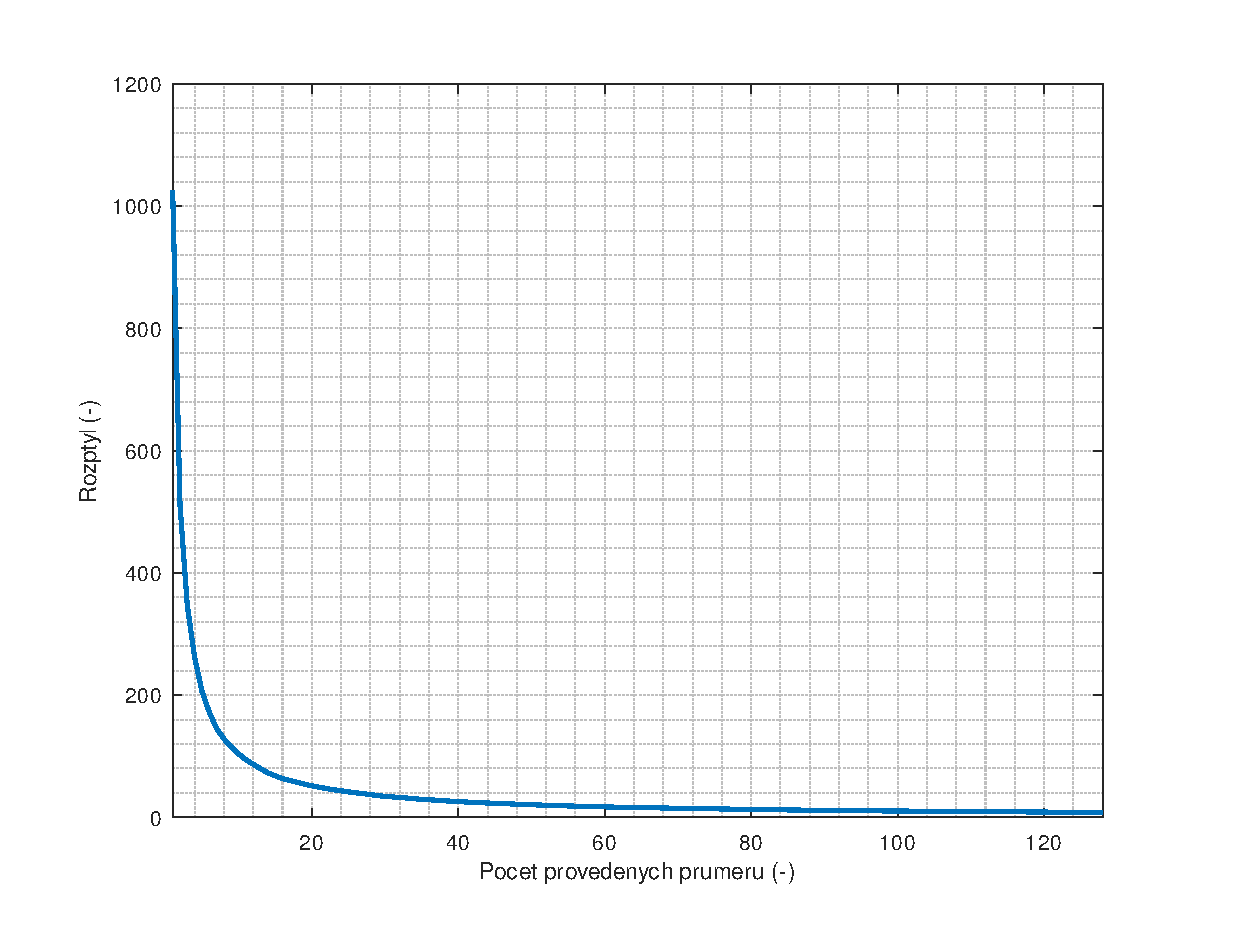
\includegraphics[width=\textwidth,keepaspectratio]{images/averaging_float_variance.eps}\caption{Závislost rozptylu na počtu provedených průměrů.}\label{averaging_variance}
\end{figure}	

Průběh této závislosti odpovídá funkci $\frac{1}{N}$, což je možné dokázat tak, že se rozptyl ve všech bodech pronásobí počtem průměrů, který danému bodu odpovídá. Na grafu \ref{averaging_float_difference_error} je vidět, že součin rozptylu s počtem průměrů je přibližně konstantní a odpovídá počátečnímu rozptylu. Diference rozptylu se pro větší počet průměrů než 16 blíží nule. Pro více než 16 průměrů, tedy polovinu směrodatné odchylky, tedy již úroveň šumu výrazně neklesá.

\begin{figure}[htbp]
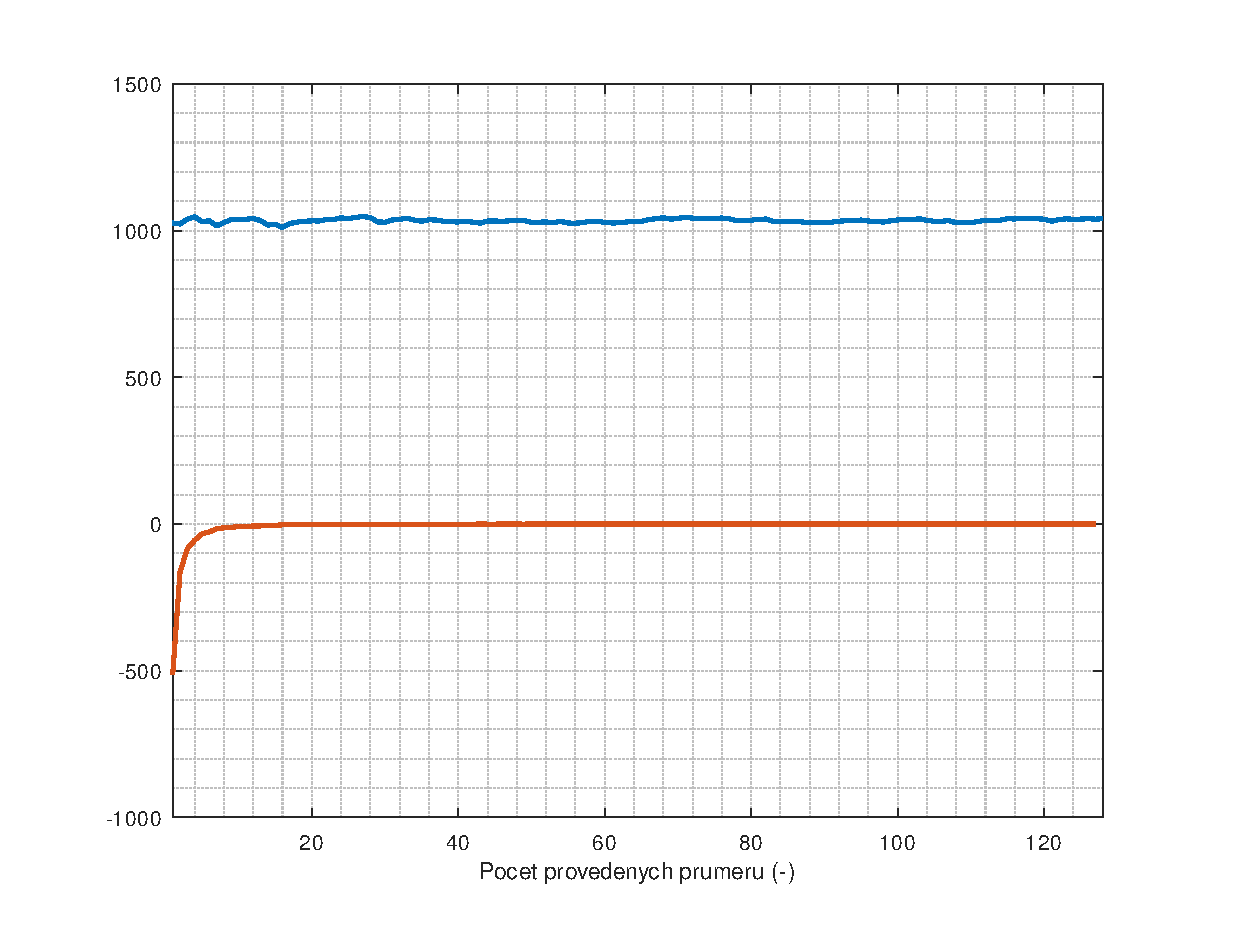
\includegraphics[width=\textwidth,keepaspectratio]{images/averaging_float_difference_error.eps}\caption{Závislost diference rozptylu (červeně) a součinu rozptylu s počtem průměrů (modře) na počtu provedených průměrů pro výpočet v plovoucí desetinné řádce.}\label{averaging_float_difference_error}
\end{figure}

V případě celočíselných výpočtů vypadá diference rozptylu podobně, ovšem ze součinu počtu průměrů a rozptylu je vidět, že závislost rozptylu na počtu průměrů neodpovídá již přesně hyperbolické funkci. Jde o vliv numerických chyb způsobovaných zaokrouhlováním výsledků. Pro větší počet průměrů než je směrodatná odchylka měřeného signálu, již znatelně stoupají numerické chyby. Význam tohoto faktu spočívá v tom, že již nestoupá odstup užitečného signálu od šumu, protože dominantním zdrojem šumu jsou chyby zaokrouhlování.

\begin{figure}[htbp]
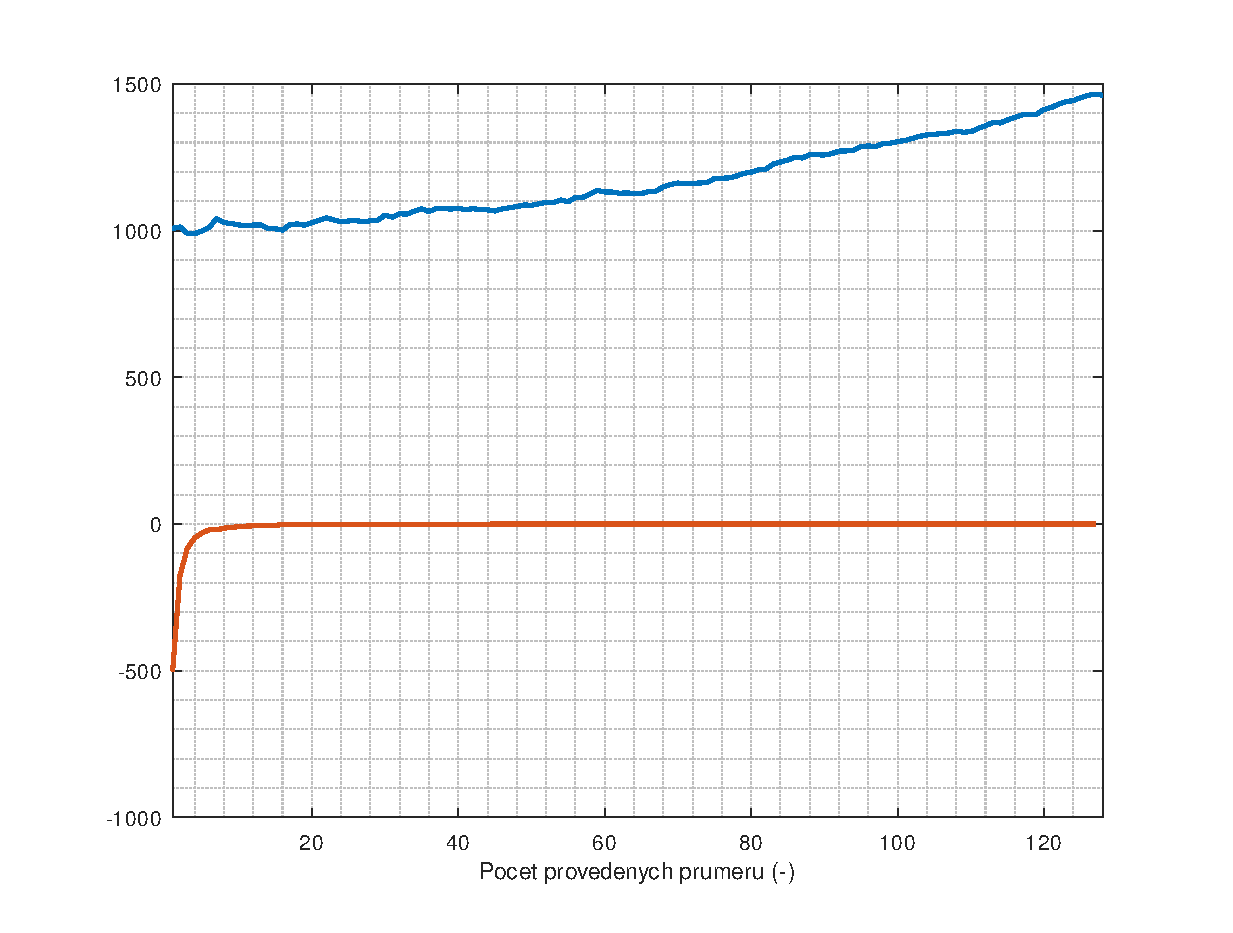
\includegraphics[width=\textwidth,keepaspectratio]{images/averaging_integer_difference_error.eps}\caption{Závislost diference rozptylu (červeně) a součinu rozptylu s počtem průměrů (modře) na počtu provedených průměrů pro celočíselné výpočty.}\label{averaging_float_difference_error}
\end{figure}

Výsledkem těchto simulací je odhad vhodného počtu průměru. Optimální počet průměrů $N$ tedy leží v rozsahu $\langle\frac{\sigma}{2}, \sigma \rangle$, kde $\sigma$ je směrodatná odchylka měřeného signálu. Po změření rozptylu měřeného signálu je tedy možné přímo odhadnout vhodný počet průměrování.

\subsection{Autokalibrace polohy budicího pulzu}
Při zapnutí fázového závěsu je fázový rozdíl mezi budicím signálem a vzorkovacím signálem náhodný. Proto je potřeba nejprve najít polohu budicího pulzu v měřených datech. Vzhledem k tomu, že není pro nedostatek RAM možné uložit celé měření a v uložených datech hledat budicí impulz, je využito přímého hledání náběžné hrany. Ta probíhá tak, že v obslužném přerušení se ukládá posledních 8 měřených vzorků, ze kterých se počítá průměr diferencí přes těchto 8 vzorků kvůli zvýšení imunity vůči šumu. Výpočet této průměrné diference je možné zjednodušit podle vzorce \ref{equation_difference_sum}. 

\begin{equation}
\begin{gathered}
	diff_{AVG8}[n]= \dfrac{1}{8} \sum_{k=0}^7 \dfrac{x[n-k]-x[n-(k+1)]}{2}= \dfrac{x[n]-x[n-8]}{16}
\end{gathered}
\label{equation_difference_sum}
\end{equation}

Pak platí, že pro průměr $n$ diferencí je potřeba spočítat jen diferenci ze dvou vzorků vzdálených o~$n$~prvků. Tato operace tedy pro každý změřený vzorek vyžaduje jedinou matematickou operaci, a tedy zabere malé množství výpočetního času, díky čemuž je možné tento výpočet umístit do obslužného přerušení. Z tohoto spočteného průměru diferencí se hledá maximum, tedy oblast s nejvyšší strmostí. Během fáze hledání náběžné hrany je mimo přerušení sledována odhadnutá poloha náběžné hrany. Pokud se tato poloha čtyřikrát v řadě ocitne v tolerančním poli $\pm256$ bodů, je tato poloha uznána jako skutečná poloha náběžné hrany. Celá tato autokalibrační fáze probíhá s odpojeným měřeným systémem.

\begin{figure}[htbp]
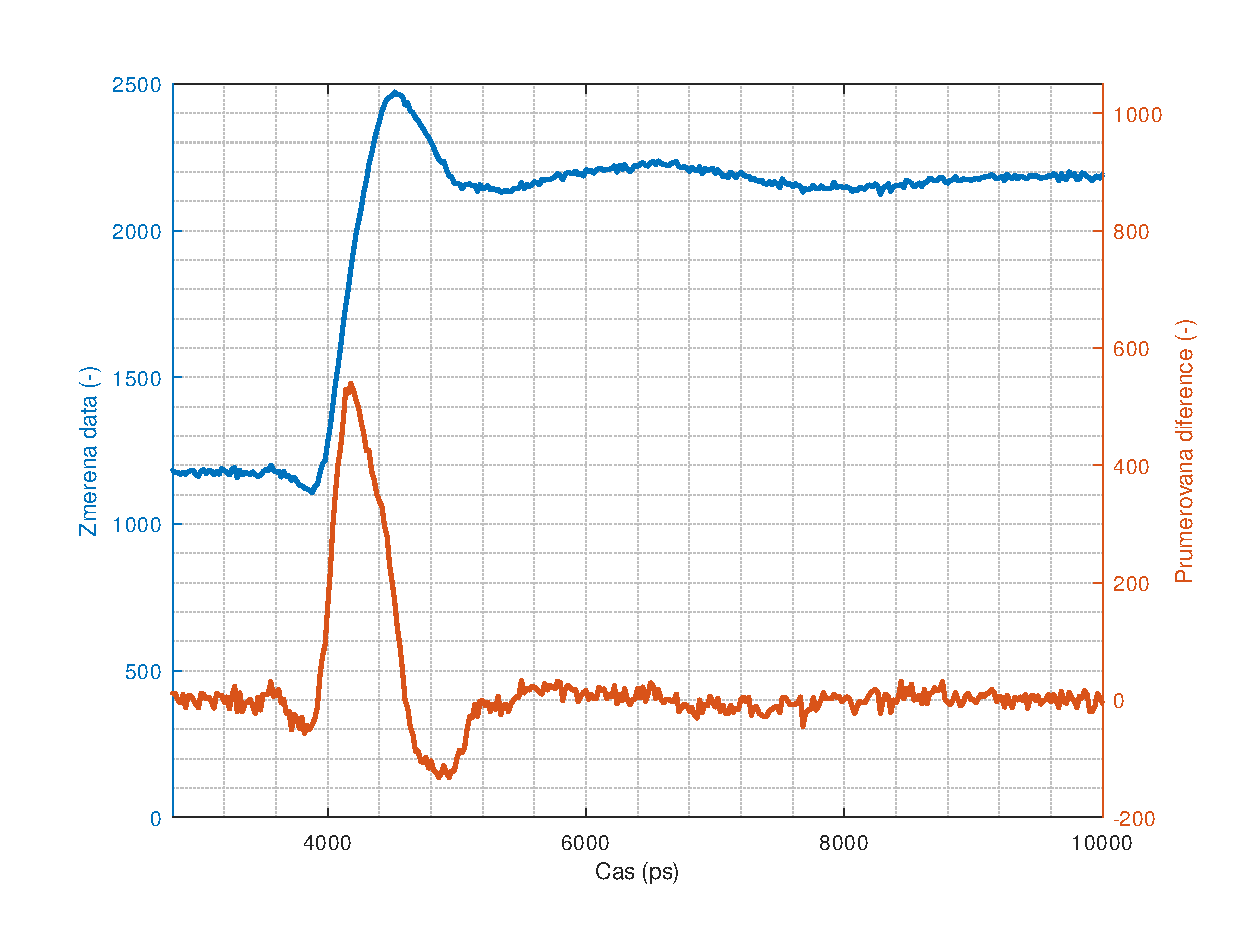
\includegraphics[width=\textwidth,keepaspectratio]{images/rising_edge_port_load.eps}\caption{Budicí pulz při připojeném standardu \quotedblbase load\textquotedblleft . Červeně je vyznačena diference při průměrování přes 8 bodů. Maximum diference odpovídá přibližně středu náběžné hrany.}\label{rising_edge_port_load}
\end{figure}

\subsection{Kalibrace polohy roviny měření}
Následně je poloha měřicího okna nastavena 512 bodů před detekovanou hranu budicího pulzu. Reflektometr čeká na zásah uživatele, je vyžadováno připojení vedení, na jehož konec se později bude připojovat měřený systém. Na konec vedení je při tomto kalibračním kroku připojený kalibr typu \quotedblbase open\textquotedblleft. Průběh v okolí budicího pulzu je osmkrát změřen a zprůměrován. Ve změřeném průběhu je v oblasti odhadnuté náběžné hrany v rovině měření změřena počáteční napětí před náběžnou hranou a konečné napětí po náběžné hraně, odhad probíhá na základě maxima, ke kterému dochází na náběžné hraně v rámci překmitu. Následně proběhne hledání bodů, kde náběžná hrana prochází \SI{20}{\percent} a \SI{80}{\percent} mezi počátečním a konečným napětím. Z polohy těchto bodů je lineárně extrapolován počátek odezvy v rovině měření tak, aby při měření již nebyla měřena část sytému před rovinou měření. Budicí impulz je tedy po tomto kroku již mimo okno měření a nadále již v měření nijak nevystupuje. Ukázková odezva kalibru \quotedblbase open\textquotedblleft{} společně s vyznačenými význačnými body je na grafu \ref{rising_edge_DUT_open}.

\begin{figure}[htbp]
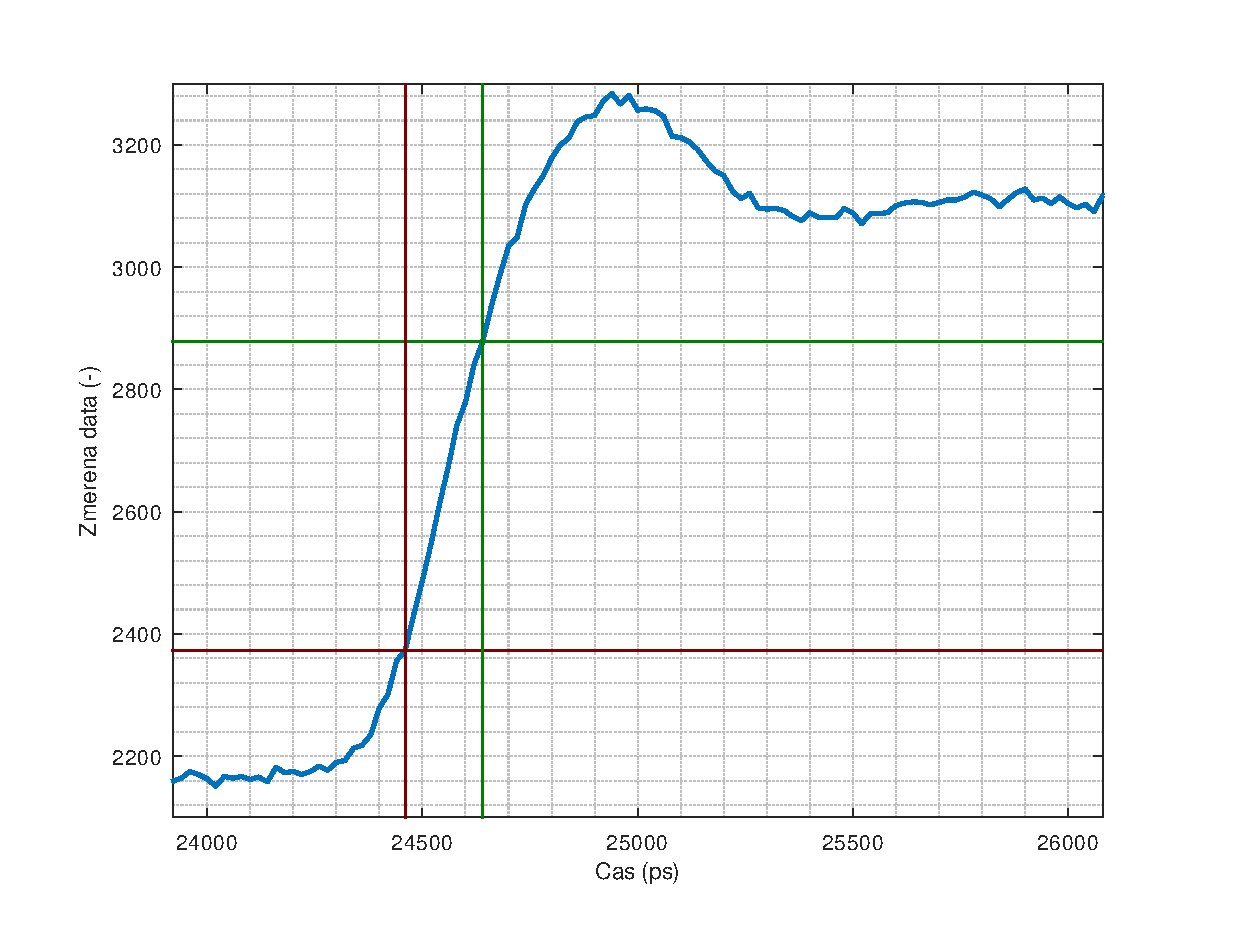
\includegraphics[width=\textwidth,keepaspectratio]{images/rising_edge_DUT_open.eps}\caption{Odezva v rovině měření při připojeném standardu \quotedblbase open\textquotedblleft , čáry vyznačují úrovně \SI{20}{\percent} a \SI{80}{\percent} náběžné hrany a jejich polohu v čase. Délka náběžné hrany v tomto úseku je \SI{180}{\pico\second}. Při měření mezi body \SI{10}{\percent} a \SI{90}{\percent} náběžné hrany je tato délka \SI{280}{\pico\second}.}\label{rising_edge_DUT_open}
\end{figure}

\section{Postup ovládání firmware}

